\chapter{The Arctic Atmosphere}
\vspace{1 cm}
\begin{spacing}{1} \begin{quote} 
\noindent \emph{Loss of multi-year sea ice and the occurrence of a seasonally ice-free Arctic Ocean by the middle of this century will result in substantial range contraction, if not the disappearance of several Arctic fish, crab, bird, and marine mammal species, including possible extinction of seals and polar bears in certain regions (high confidence).} \end{quote}
\hspace{6 cm} - Intergovernmental Panel on Climate Change (IPCC) \\
\hspace*{6.7 cm} Sixth Assessment Report, August 2021  
\end{spacing}
\doublespacing
\section{The Arctic and Climate Change}
The largest impacts of climate change are those seen in the Arctic. Over the past two decades, Arctic temperatures have increased by more than 2 times the global rate \citep{IPCC:14}. Changes occurring in the Arctic modify the atmospheric circulation, impacting both cloudiness and radiation at the surface \citep{zhang:2008}.
 
Arctic amplification is a series of mechanisms in which the polar regions undergo positive feedback loops which can change the energy balance at the surface. Arctic amplification includes the ice-albedo effect, which amplifies temperature increases due to greenhouse gas emissions by melting sea ice. As sea ice melts, the albedo of the surface decreases, resulting in more solar energy absorption. As the surface absorbs more solar energy, it warms, increasing Arctic air temperatures, which melts additional sea ice. This is a key example of a positive feedback loop \citep{ipcc_techsum}. A second example of Arctic amplification occurs when permafrost thaws, releasing stored methane into the atmosphere. This increase in atmospheric methane mixes globally, and increases the greenhouse effect everywhere, further increasing permafrost melt. While this is not the focus of this study, it is important to note and can impact global temperatures. To fully understand Arctic climate change, it is crucial for scientists to study this region and the physical processes that contribute to Arctic amplification.

Arctic climate change heavily impacts marine life, indigenous people, and coastal ecosystems \citep{ipcc_techsum}.  Beyond these local effects, changes in Arctic sea ice can also cause irreversible changes in the atmospheric and oceanic circulation. Many of the Coupled Model Intercomparison Project Phase 5 (CMIP5) models indicate that within the next few years, the Earth may experience a completely ice-free Arctic during the summer \citep{stroeve:2018}.

Sea ice has been declining at an increasing rate throughout the last decade due to lengthened melt seasons replacing multi-year sea ice  with thin, first-year sea ice \citep{meier:2014}. Multi-year sea ice can be defined as sea ice that does not completely melt in the summer. Conversely, first-year sea ice melts completely each summer and re-freezes the following winter. \citet{wunderling:2020} found that 55$\%$ of the additional warming in the Arctic was a result of the ice-albedo feedback. The rest is attributed to a change in lapse rate and cloud properties resulting in increased surface heating. Overall, these changes have resulted in an ice loss of approximately 3.4$\%$ per decade. Multi-year sea ice has decreased from 59$\%$ of the ice pack to 28$\%$ in 2018 and continues to decrease \citep{stroeve:2018}. The fraction of first-year ice has increased as a result. As a consequence of this, there is a need to fully understand atmosphere-ocean interactions over first-year ice. This movement toward a new ice regime has been referred to as a shift toward a new climate state in the Arctic \citep{verlinde:2007}. 

\section{Surface Energy Budget}
The surface energy budget can influence ice growth or melt. A study done using results from the Surface Heat Budget of the Arctic Ocean (SHEBA, described in Section 1.3) field experiment over sea ice shows that the ice and snow thickness have significant impacts on the surface temperature and, as a result, the surface energy budget, due to the changes in heat transfer through the snow and ice \citep{hines:2015}. Additionally, the surface energy budget is often misrepresented in models due to an underestimation of cloud cover, resulting in downward longwave radiation biases \citep{inoue:2008}. Eq. \ref{eq:qnetintrointro} and \ref{eq:r} show the net radiation and surface energy budget equations.

\begin{equation}\label{eq:qnetintrointro}
Q_{net} = (Q_{sw \downarrow} - Q_{sw \uparrow}) + (Q_{lw \downarrow} - Q_{lw \uparrow})
\end{equation}
\begin{equation}\label{eq:r}
R = Q_{net} + H_{s} + H_{l}
\end{equation}

$Q_{sw}$ and $Q_{lw}$ are the shortwave and longwave radiative fluxes, respectively, with the arrow denoting upward ($\uparrow$) vs downward ($\downarrow$) flux, $R$ is the residual flux, including heat transfer through the ice and heat storage, and $H_{s}$ and $H_{l}$ are the sensible and latent heat fluxes. While net radiative flux can easily be measured or estimated given temperature profiles and cloud cover, values such as the sensible and latent heat fluxes are not as straightforward to estimate. Models often have skill in one value but have large compensating errors in other values. These values are heavily influenced by both the clouds and the near-surface boundary layer structure \citep{tjernstrom:2005}.

\subsection{Clouds: Longwave and Shortwave Radiation}
Properties such as proximity to melt ponds/open water, the shape of the snow crystals, and snow depth, can all influence how clouds modify surface radiation. Due to complexities in cloud feedbacks and the underlying surface, there are a variety of ways models handle cloud formation and properties. Arctic atmospheric models, while key to understanding cloud processes, are not perfect and still have trouble quantifying these processes. 

A key feedback mechanism in the arctic regions is the cloud radiation feedback, which, unlike other Arctic amplification feedbacks, can be either positive or negative depending on influences such as the cloud properties and sun angle. This process applies all over the globe, but due to the high surface albedo and lack of atmospheric moisture, it has a greater potential to influence the surface radiation budget in the Arctic. Further research is still necessary to quantify the exact influence. When clouds are lower in the atmosphere or are more optically thick they emit more longwave radiation. However, a cooler cloud, one higher in the atmosphere, or optically thin, would radiate less longwave radiation, but still more than under clear-sky conditions. This is an example of how clouds can warm the surface. Clouds can cool the surface as a result of their shortwave impact. The higher the cloud's albedo (higher optical thickness and droplet size), the more shortwave radiation is reflected away, not reaching the surface, and not being included in the surface energy budget. \citet{intrieri:2002} studied the radiative influence of clouds at SHEBA and found that, for their location northeast of Alaska, the net cloud effect was to warm the surface through most of the year. There was only a short two-week period in the middle of the summer, when the location was getting the most direct solar radiation and had the lowest surface albedo, when clouds had a cooling influence by reflecting shortwave radiation away from the surface. 

Cloud radiative forcing (CRF) is often used to quantify the impacts of clouds on surface radiation. This is defined in Eq. \ref{eq:crf}, but can be conceptually understood as the difference between the surface radiation in the absence of clouds ($Q_{clear}$) and the actual (or all-sky) radiation ($Q_{all} = Q_{net}$). A large positive (negative) cloud radiative forcing indicates surface warming (cooling) due to cloud radiative influence. 

\begin{equation}\label{eq:crf}
CRF = Q_{all} - Q_{clear} 
\end{equation}

\subsection{Sensible and Latent Heat Flux}
The near-surface planetary boundary layer (PBL) is often strongly stable in the Arctic due to significant surface longwave radiative cooling that is not compensated for by other energy sources. This is mainly due to the low level of solar heating as a result of little incoming sunlight much of the year and generally high surface albedo. Additionally, the latent heat of phase change in the surface during the melt season acts to cool the air closest to the surface, creating a stable boundary layer. Global models, however, often have a difficult time simulating these strongly stable conditions, and either form a PBL not stable enough or too stable for actual conditions. Regional models are generally better than this and can be used to improve larger-scale models, but there is still a need for further model improvement \citep{tjernstrom:2005}. 

\section{Arctic Measurements}
One of the first major experiments studying meteorology and ice dynamics in the Arctic Ocean took place between 1975 and 1976. This experiment, The Arctic Ice Dynamics Joint Experiment (AIDJEX), was led by the University of Washington and consisted of four ice camps with surrounding buoys \citep{untersteiner:1980}. Taking measurements over sea ice is both dangerous and difficult as deployment and maintenance is nearly impossible without the aid of a ship. Another way of taking in-situ measurements includes floating buoys, but the measurement capabilities of buoys are limited by the lack of available onboard power. Research vessels are utilized for their ability to provide power, transportation, and housing for scientists while observing the Arctic.

A series of ship-borne experiments took place between 1991 and 2001: the International Arctic Ocean Experiment (AOE) (1991), AOE-96 (1996) \citep{tjernstrom:2004}, SHEBA (October 1997 - October 1998) \citep{uttal:2002}, and AOE (2001). The earlier two AOE focused on atmospheric aerosols and did not include vertical profiles of atmospheric structure or ice characteristics. The 2001 AOE experiment focused more extensively on meteorological variables \citep{tjernstrom:2004}. SHEBA had a larger array of meteorological instruments, observing both the cloud properties and the surface energy budget over sea ice for an entire year \citep{uttal:2002}. Before the Norwegian Young Sea Ice Campaign (N-ICE2015 or N-ICE) took place in January through June of 2015, SHEBA was the most recent experiment to observe these atmospheric properties. 

Other experiments since SHEBA, such as the Arctic Clouds in Summer Experiment (ACSE) \citep{sotiropoulou:2016}, and the Mixed-Phase Arctic Cloud Experiment \citep{verlinde:2007} have not observed winter or took place over a shorter duration than N-ICE. Prior to SHEBA, field experiments such as the Seasonal Ice Zone Experiment, Coordinated Eastern Arctic experiment, Marginal Ice Zone Experiments, Arctic Ice Dynamics Joint Experiment, and the Soviet and Russian drifting stations \citep{vihma:2005, kahl:1999} that collected meteorological and radiation data over Arctic sea ice either covered a small area or had poor temporal resolution. However, these studies have used observations of cloud cover, albedo, and cloud properties to provide estimates of the surface energy budget. Comparing SHEBA data to these estimates showed that during transition seasons (September, October, November, March, and April), the SHEBA time period had larger incoming longwave radiation and a smaller magnitude of shortwave radiation, sensible heat flux, and latent heat flux compared to other studies. This could be caused by a higher frequency of warm air masses, an increase in cloud cover, or a combination of both \citep{persson:2002}. 

SHEBA took place onboard a Canadian Coast Guard ice breaker, the Des Groseillers, in the Beaufort Sea north of Alaska from 1997 to 1998 \citep{uttal:2002, shupe:2004}. The ship sailed north from Alaska and was intentionally frozen into the sea ice and allowed to drift with the ice \citep{uttal:2002}. Helicopter flights also surveyed the area to document the ice conditions surrounding the ship and a tethered balloon was utilized to observe the boundary layer conditions. The primary goals of this experiment were to observe the changes occurring in the surface energy budget over sea ice as the polar regions undergo global warming with the hope that these observations can give both context to the poorly understood mechanisms occurring under these never-before-observed conditions and to provide observations to validate and improve general circulation models in the Arctic \citep{uttal:2002}. Particular focus was on ocean-ice-atmosphere feedback, such as the ice-albedo and cloud-radiation feedback during the entire annual cycle. 

The ice pack SHEBA was frozen into varied in thickness from 1.8 $m$ (October) to 2.6 $m$ (June) and was classified as multiyear sea ice, indicating this ice pack had not completely melted the previous summer. Snowpack was also observed on the ice throughout the experiment, reaching a maximum depth in June, when 30 $cm$ of snow fell but melted quickly in the following days \citep{uttal:2002}. Multi-year sea ice is becoming less prominent in the polar regions, and first-year sea ice is beginning to dominate the Arctic. This shift away from the conditions seen at SHEBA and toward thinner, first-year sea ice motivated N-ICE2015, which observed conditions over young sea ice and is described in Chapter 2 \citep{graham:2017}. 

During the start of SHEBA, the western Arctic had an anomalously large amount of multi-year ice. In addition, the autumn upper ocean had a lower salinity and warmer temperature than expected, indicating a larger ocean heat flux than was typical of the area during the summer. Comparing SHEBA data to estimates from other field experiments showed that during transition seasons (September, October, November, March, and April), SHEBA observed incoming longwave radiation that was 2 to 45 $Wm^{-2}$ more than other studies. This could be caused by either an increase in the number of warm air masses over SHEBA or an increase in cloud cover \citep{persson:2002}. SHEBA was an important field experiment that filled many gaps in our understanding of cloud and radiation processes. One of the most important findings from SHEBA was that, even at temperatures well below freezing, mixed-phase clouds occurred often. 

SHEBA took place over thick, multi-year sea ice. The Arctic is shifting toward a new regime dominated by thin, first-year sea ice, so observations over first-year sea ice are necessary to understand these increasingly more dominant conditions. Since N-ICE, there has been one major field campaign with the goal of observing the Arctic climate system onboard an icebreaker ship \citep{shupe:2020}. The Multidisciplinary drifting Observatory for the Study of Arctic Climate (MOSAiC) was a year-long field expedition that took place in the central Arctic in 2019. Much like SHEBA, MOSAiC took place further north than N-ICE and was primarily over multi-year sea ice \citep{martin:2020}. This shift toward an Arctic dominated by first-year sea ice and the lack of measurements over first-year sea ice are the primary motivations of N-ICE. Chapter 2 gives details of N-ICE, including instruments deployed and driving questions.

\section{Dissertation Outline and Attributions}
\newline 
\noindent This dissertation aims to:
\begin{enumerate}
\item Compare atmospheric measurements to models (Chapter 3)
\item Investigate combinations of cloud microphysics and boundary layer physics options within WRF (Chapter 3)
\item Explore the cloud conditions seen at N-ICE (Chapter 4)
\item Investigate the effects of turbulent fluxes and clouds on young sea ice (Chapter 5 and 6)
\item Make recommendations for improving the Polar WRF model (Chapter 6 and 7)
\end{enumerate}

\begin{figure}[b!]
    \centering 
    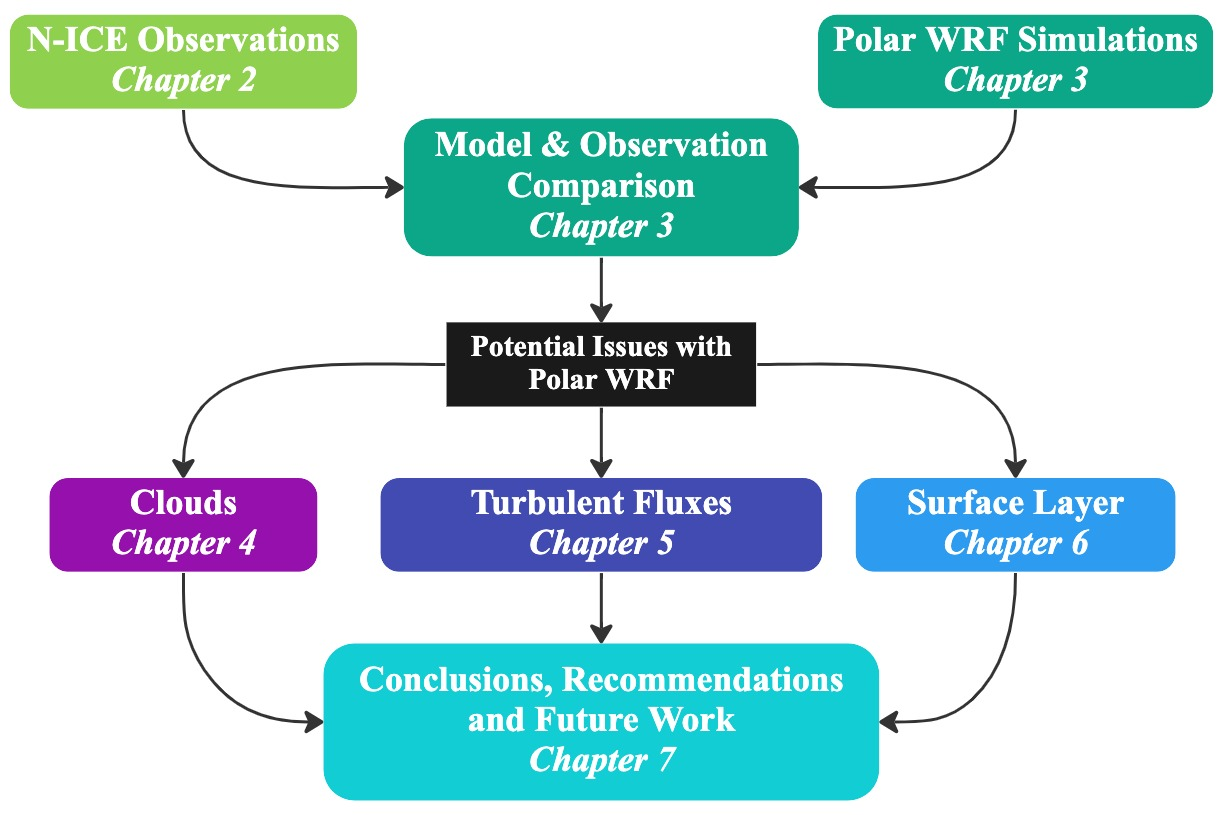
\includegraphics[width=1\linewidth]{figures/flowchart.jpg}
    \caption[Flowchart of dissertation chapters.]{A flowchart showing how each chapter of this dissertation ties together. Boxes are colored by chapter.}
    \label{fig:flowchart}
\end{figure}

Figure \ref{fig:flowchart} is a flowchart showing all of the following chapters and how they tie together. Chapter 2 describes the general aspects of the N-ICE field campaign that are common to all subsequent chapters. 

Chapter 3 presents model simulations performed by the Polar Weather Research Forecasting (Polar WRF) model and compares the various schemes used for the planetary boundary layer and cloud microphysical properties. The model simulations are summarized in terms of how well they compared with the N-ICE measurements. This work was completed on the Cheyenne \citep{cheyenne} supercomputer by Murphy with guidance from Dr. Keith Hines. This chapter was written with the intention to submit as a publication to the American Geophysical Union (AGU) Journal of Advances in Modeling Earth Systems.

Chapter 4 provides detail on the measurements of cloud radiative properties during N-ICE and how they relate to the Polar WRF simulations. The analysis for this chapter was completed by Murphy, with LiDAR processing and section 4.3.1 being completed by Dr. Robert Stillwell. Dr. Von Walden and Dr. Stephen Hudson were advisors on this research. This chapter was written for submission to the Journal of Geophysical Research (JGR) Atmospheres journal.

Chapter 5 compares the turbulent fluxes observed at N-ICE to fluxes calculated using the Maximum Entropy Production method and a bulk flux algorithm. These methods of calculating fluxes depend on exchange coefficients and surface stability, which are also explored in Chapter 5. All research, coding, analysis, and writing was completed by Sarah with advice from Drs. Hailong Wang and Von P. Walden. This research was done in collaboration with Pacific Northwest National Laboratory as part of the Department of Energy's Office of Science Graduate Student Research Program (DOE SCGSR). 

The equations used in the Polar WRF model are described in detail in Chapter 6, comparing them to the methods of calculating flux in Chapter 5. This chapter uses the measurements described in Chapter 4, the equations explored in Chapter 5, and the modeling schemes detailed in Chapter 3 to conduct sensitivity studies to changes within WRF. This work will also be submitted to AGU's Journal of Advances in Modeling Earth Systems.

Chapter 7 wraps up this dissertation by summarizing the findings in Chapters 3 through 6. This chapter also includes suggestions for changes to the WRF model and topics for future research, including how the cloud properties could be further explored to improve radiation in the model.

In addition to the work presented in this dissertation, Murphy also completed data processing of the flux data. Appendix B documents the process of determining the sensitivity of LiCor's EddyPro eddy covariance (EC) flux processing software results to gaps in the input datasets and a method for artificially filling these gaps in the most accurate way to represent missing data. These data were published as a dataset \citep{niceflux} and in a publication \citep{walden:2017}, in which Murphy is a co-author.